\subsection{Measuring Master}
\subsubsection{Vorstellung}
Die App \mm{} von der Bosch GmbH ist im Google Play-Store unter der Rubrik ``Effizienz'' aufgelistet.
Bei der vorliegenden App handelt es sich um die Version \emph{1.3.1}, welche am 30. November 2017 aus dem Play-Store\urlnote{https://play.google.com/store/apps/details?id=com.bosch.measuringmaster&hl=de}{30.11.2017} runtergeladen wurde.
Selbst beschreibt der App-Hersteller die App wie folgt \citep{BoschMM}:

\begin{quote}
  ``Measuring Master ist eine multifunktionale App, die es ermöglicht, Aufmaße, Grundrisse und Temperaturmesswerte an einem Ort zu dokumentieren und zu verwalten.\\
  Die App ist besonders geeignet für Architekten, Maler, Bodenleger, Heizungsbauer und Elektriker, aber auch alle anderen Handwerker profitieren von der umfangreichen Funktionalität''
\end{quote}

\noindent
Nach dem Start der Applikation bietet sich die Möglichkeit ein neues Projekt anzulegen, oder bereits vorhandene Projekte zu bearbeiten.
Sobald das gewünschte Projekt ausgewählt wurde, kann der Benutzer durch Ausklappen des Menüs an der linken Seite die Funktionen der App (siehe \autoref{fig:bmenu}) der App sehen. \\

\begin{figure}[h]
  \begin{subfigure}[t]{0.45\textwidth}
    \centering
    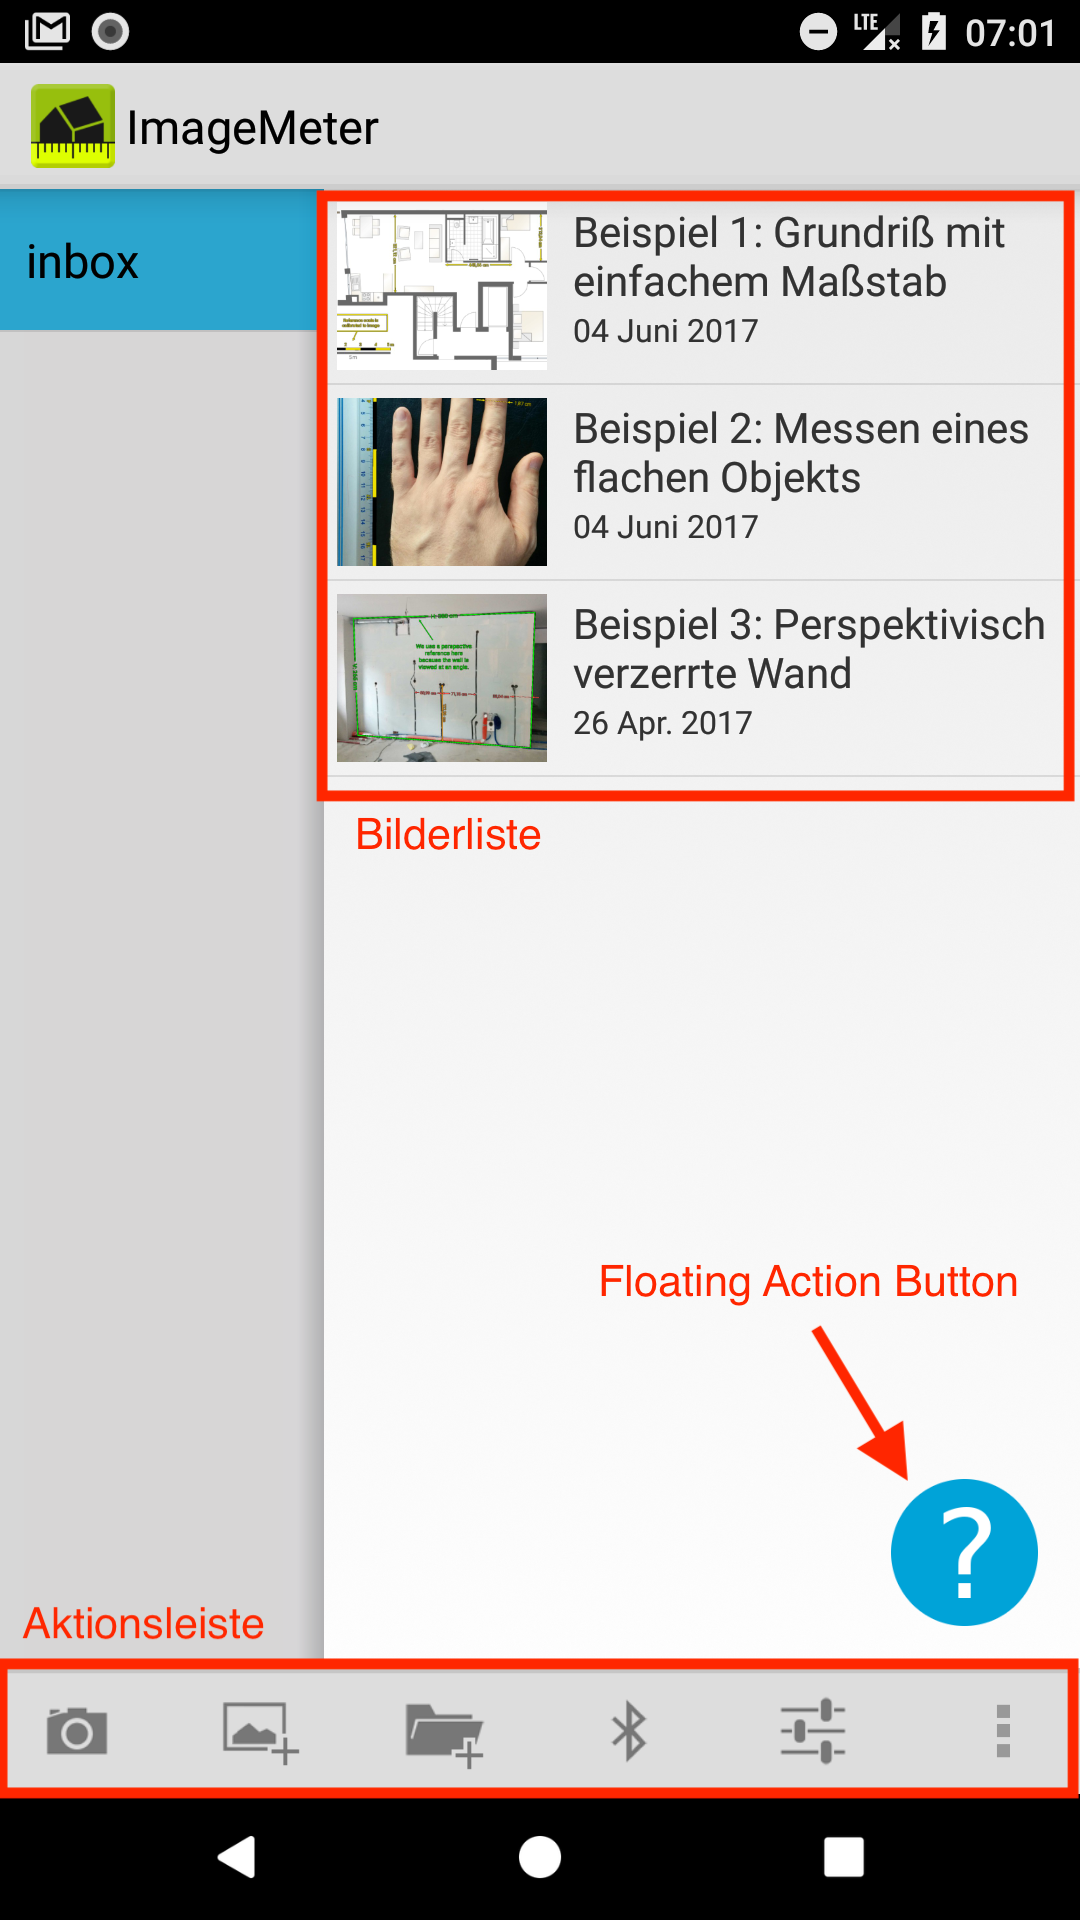
\includegraphics[keepaspectratio, width=\textwidth]{bosch/menu}
    \caption{Navigationsmenü}\label{fig:bmenu}	
  \end{subfigure}
  ~
  \begin{subfigure}[t]{0.45\textwidth}
    \centering
    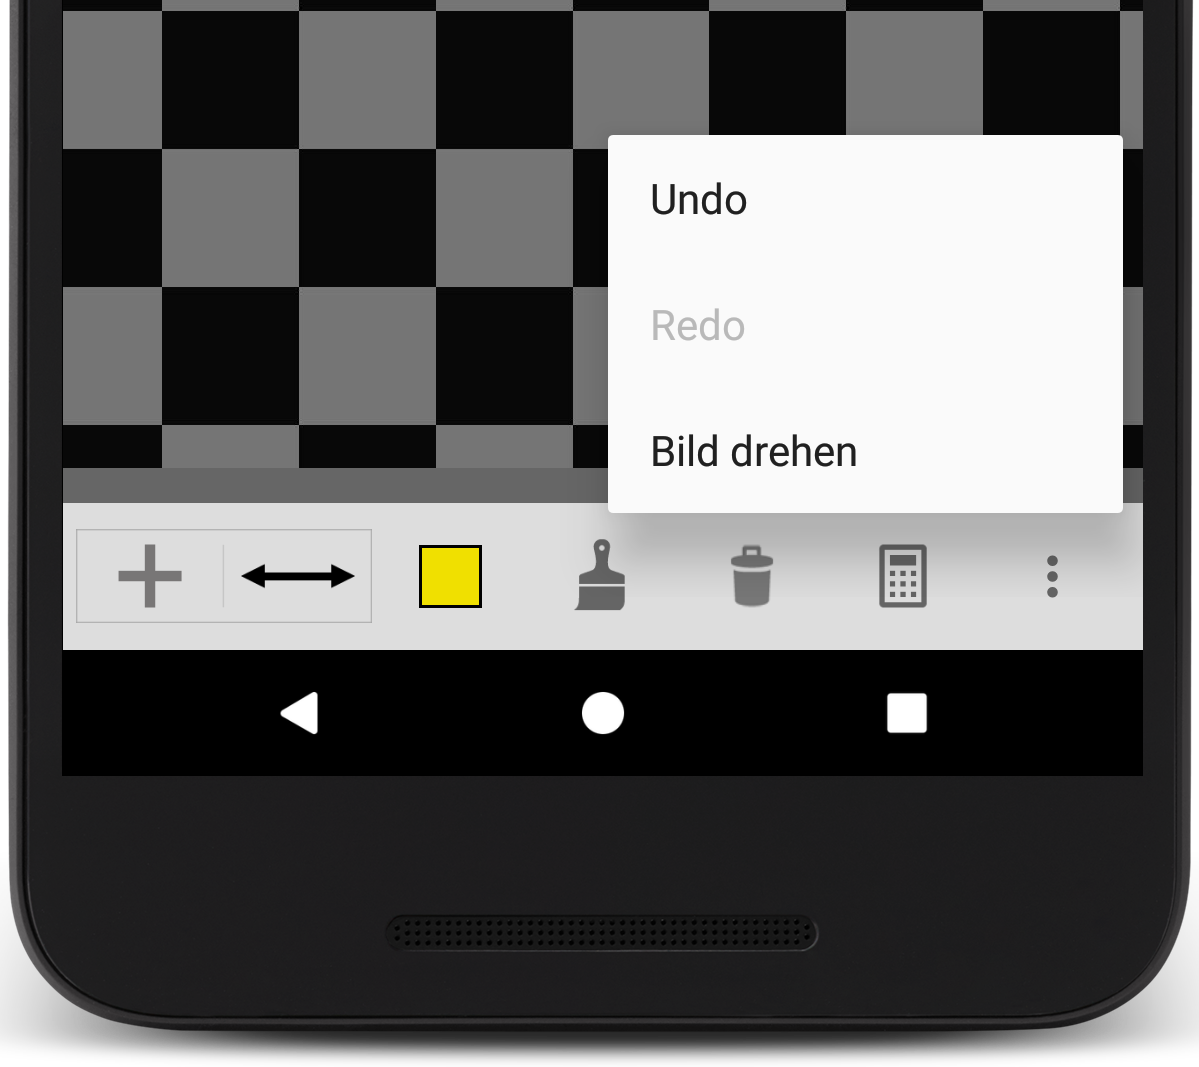
\includegraphics[keepaspectratio, width=\textwidth]{bosch/bar}
    \caption{Aufmaß-Funktion}\label{fig:bbar}
  \end{subfigure}
  \centering
  \caption{\mm{} bei ausgeklapptem Navigationsmenü und in der Aufmaße-Funktion}
\end{figure}

Im Folgenden wird der Menüpunkt ``Aufmaße'' und die damit verbundene Funktionalität weiter vorgestellt und evaluiert.
So bietet sich dem Benutzer nach Auswahl der Aufmaße-Funktion die Möglichkeit, beliebige Bilder mit Messwerten zu beschriften.
Hierzu können die Bilder entweder direkt aus der Galerie importiert, oder mit der Kamera aufgenommen werden.
Sobald der Nutzer den Foto-Import erfolgreich abgeschlossen hat, öffnet sich eine neue Benutzeroberfläche, die das zuvor ausgewählte Bild und weitere Bedienelement zeigt (siehe \autoref{fig:bbar}). \\

In dieser Oberfläche kann der Benutzer vier verschiedenen Formen (Linie, Viereck, Winkel, Freiform) in das Bild anzeichnen und über einen Klick auf die gewünschte Form die zugehörigen Messwerte eintragen.
Hierbei bietet die App zusätzlich die Funktion, ein Laserentfernungsmesser mit der App zu verbinden.
Dieser ermöglicht das Übertragen der gemessenen Distanzen über eine Bluetooth-Schnittstelle direkt an die App. \\

Um das annotierte Bild außerhalb der App weiter zu benutzen, bietet diese den Export als \emph{PDF} oder \emph{JPEG} an.
Die exportierte \emph{PDF} enthält im Gegensatz zu der \emph{JPEG} zusätzlich zu dem annotierten Bild auch noch eine Tabelle mit allen eingetragenen Messwerten \autoref{fig:bexport}. 
Zudem lassen sich die Bilder in der App speichern und zu einem späteren Zeitpunkt weiter bearbeiten.

\begin{figure}[h]
  \centering
  \shadowbox{
    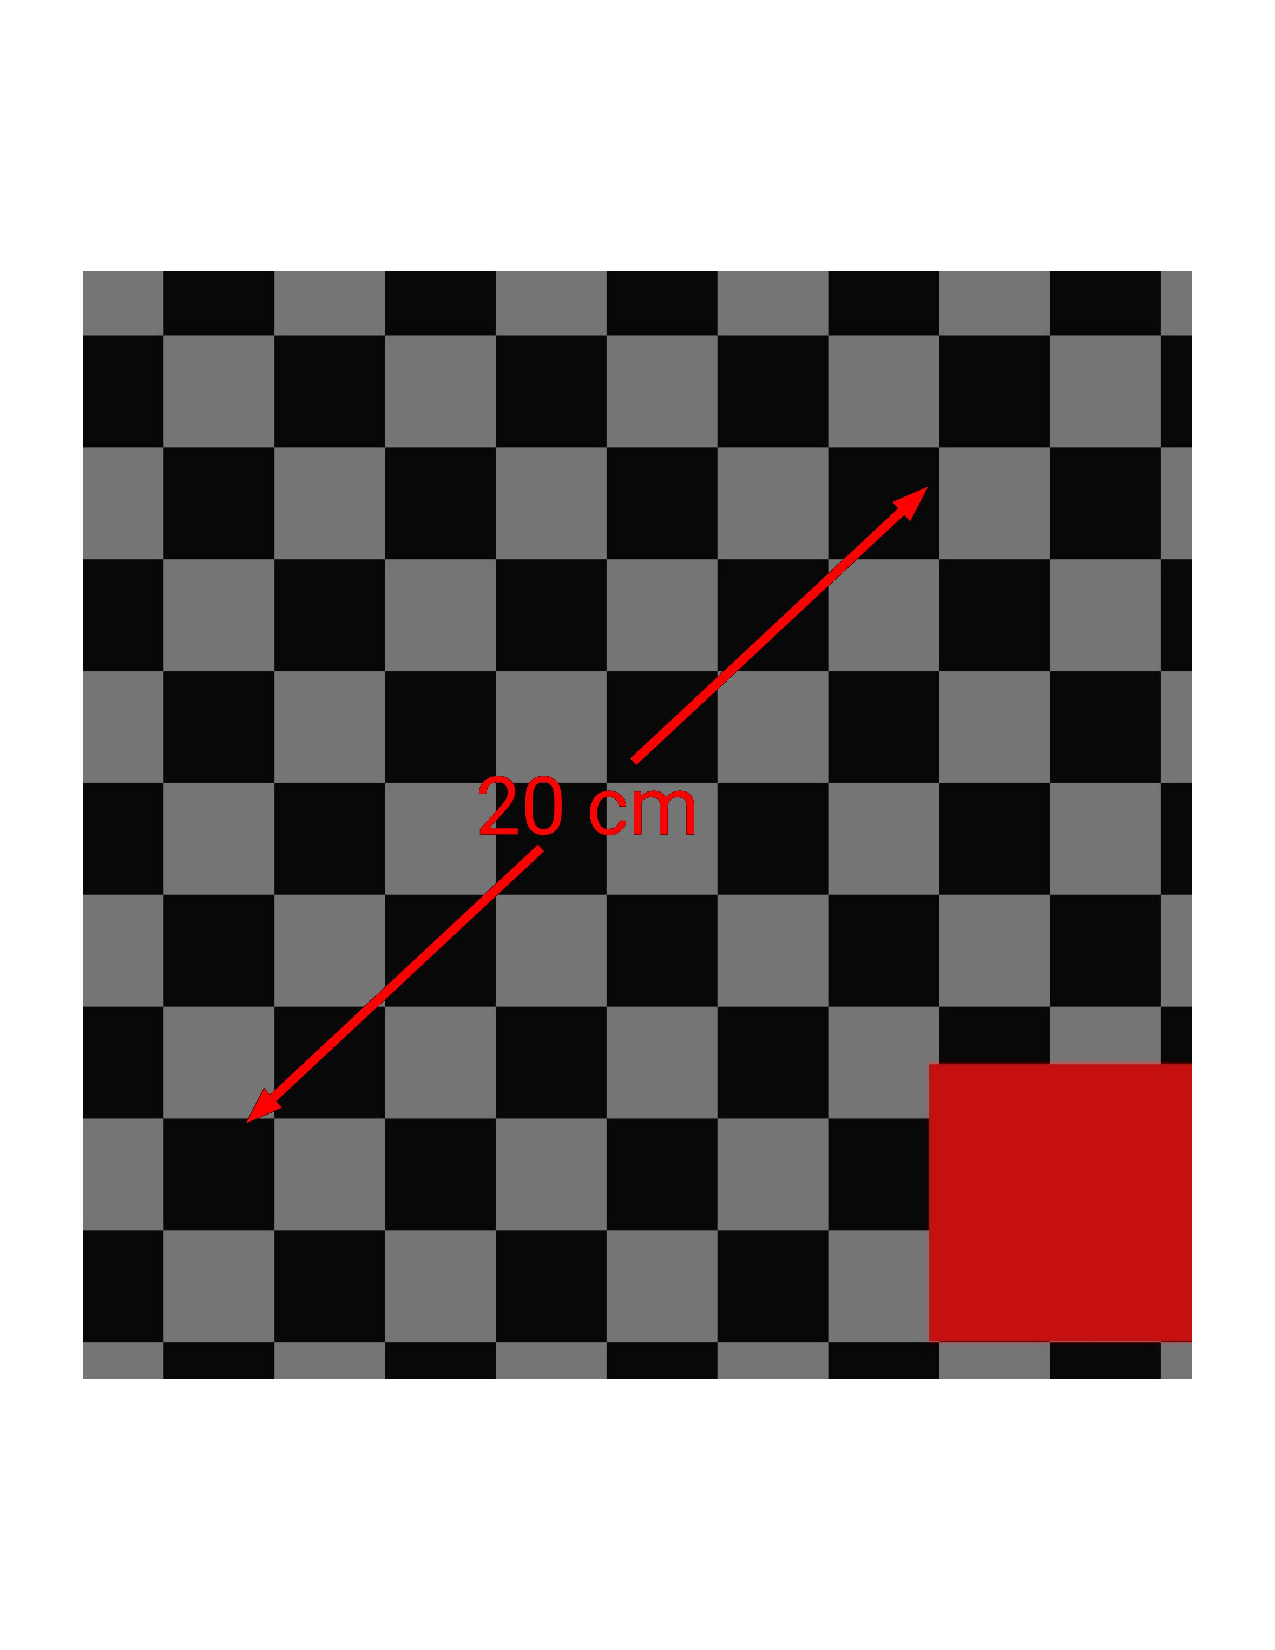
\includegraphics[keepaspectratio, width=\textwidth]{bosch/export}
  } 
  \caption{Exportierte PDF}\label{fig:bexport}
\end{figure}

\subsubsection{Evaluation}
Durch die Anzeige einer Statusleiste am unteren Bildschirmrand (siehe \autoref{fig:bbar}) gibt die App dem Benutzer zu jeder Zeit eine klare und sichtbare Rückmeldung über den aktuellen Systemzustand (Nielsen~\autoref{itm:N1}). \\

Zusätzlich bietet der erklärender Text im oberen Bereich des Bildschirms (siehe \autoref{fig:bbar}) eine konkrete Hilfestellung zu den möglichen Aktionen, die der Benutzer im aktuellen Systemzustand ausführen kann.
So fungiert der Satz ``Linie wählen oder zeichnen'' in \autoref{fig:bbar} gleichzeitig als Hilfestellung und Aufforderung an den Nutzer eine der beiden Aktionen auszuführen.
(Nielsen~\autoref{itm:N10}). \\

Darüber hinaus kann der Nutzer über ein Undo- bzw. Redo-Symbol in der Menüleiste (siehe \autoref{fig:bbar}) fehlerhafte Eingaben rückgängig machen oder rückgängig gemachte Aktionen wiederholen (Nielsen~\autoref{itm:N3}).
Dadurch, dass alle Menüpunkte, die im aktuellen Systemzustand nicht ausgeführt werden können, ausgegraut dargestellt werden, werden Fehler präventiv vermieden (siehe \autoref{fig:bicons}).
So lassen sich Formen erst dann löschen, wenn diese zuvor markiert wurde, oder Aktionen rückgängig machen, wenn zuvor eine Benutzeraktion stattgefunden hat (Nielsen~\autoref{itm:N5}). \\

\begin{figure}[h]
  \centering
  
\includegraphics[keepaspectratio, width=\textwidth]{bosch/icons}
  \caption{Menüleiste bei ausgewählter Form und vorheriger Zeichen-Aktion}
  \label{fig:bicons}
\end{figure}

Sollte die App doch in einen Fehlerzustand gelangen, wie bspw. durch den Import eines beschädigten Bildes, wird ein \emph{Toast}\urlnote{https://developer.android.com/guide/topics/ui/notifiers/toasts.html}{30.11.2017} angezeigt (siehe \autoref{fig:btoast}).
Dieses \emph{Toast} gibt dem Nutzer eine Information darüber, was zum Fehler geführt hat (Nielsen~\autoref{itm:N9}).

\begin{figure}[h]
  \centering
  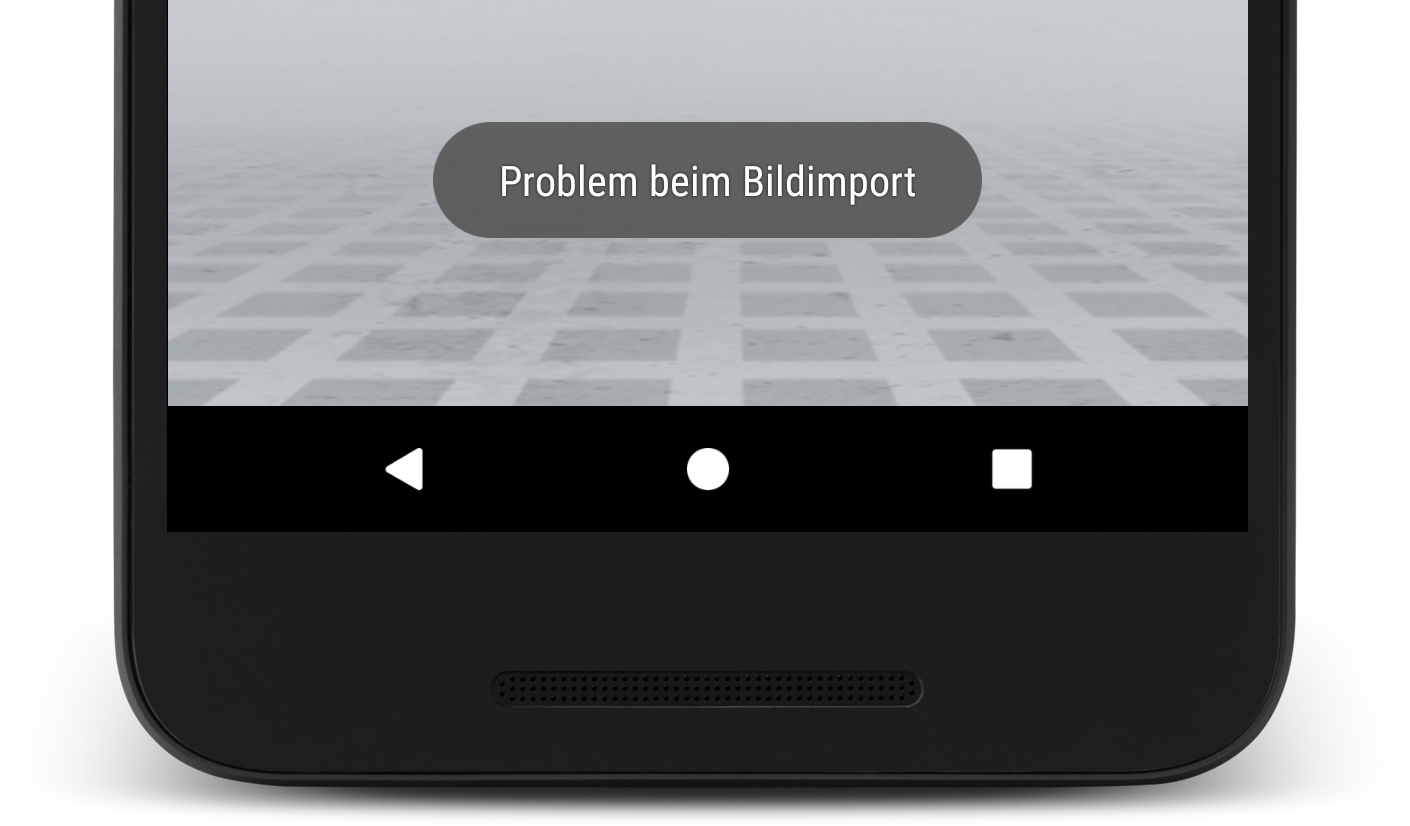
\includegraphics[keepaspectratio, width=0.5\textwidth]{bosch/toast}
  \caption{\emph{Toast} beim Import eines beschädigten Bildes}
  \label{fig:btoast}
\end{figure}

Durch die konsistente Benutzung intuitiv verständlicher Icons lassen sich die dahinter befindlichen Aktionen ohne große Anstrengung erkennen.
Dieser Punkt wirkt sich positiv auf das Nutzungserlebnis der App aus, da sämtliche Icons nicht zuerst auswendig gelernt werden müssen.
So dient zum Beispiel das Mülleimer-Icon in der Menüleiste (siehe \autoref{fig:bicons}) sowohl im Zeichen- als auch im Text-Modus als Löschfunktion der markierten Form bzw. des ausgewählten Textes (Nielsen~\autoref{itm:N4} \& \autoref{itm:N6}). \\

\begin{wrapfigure}{R}{0.4\textwidth}
  \centering
  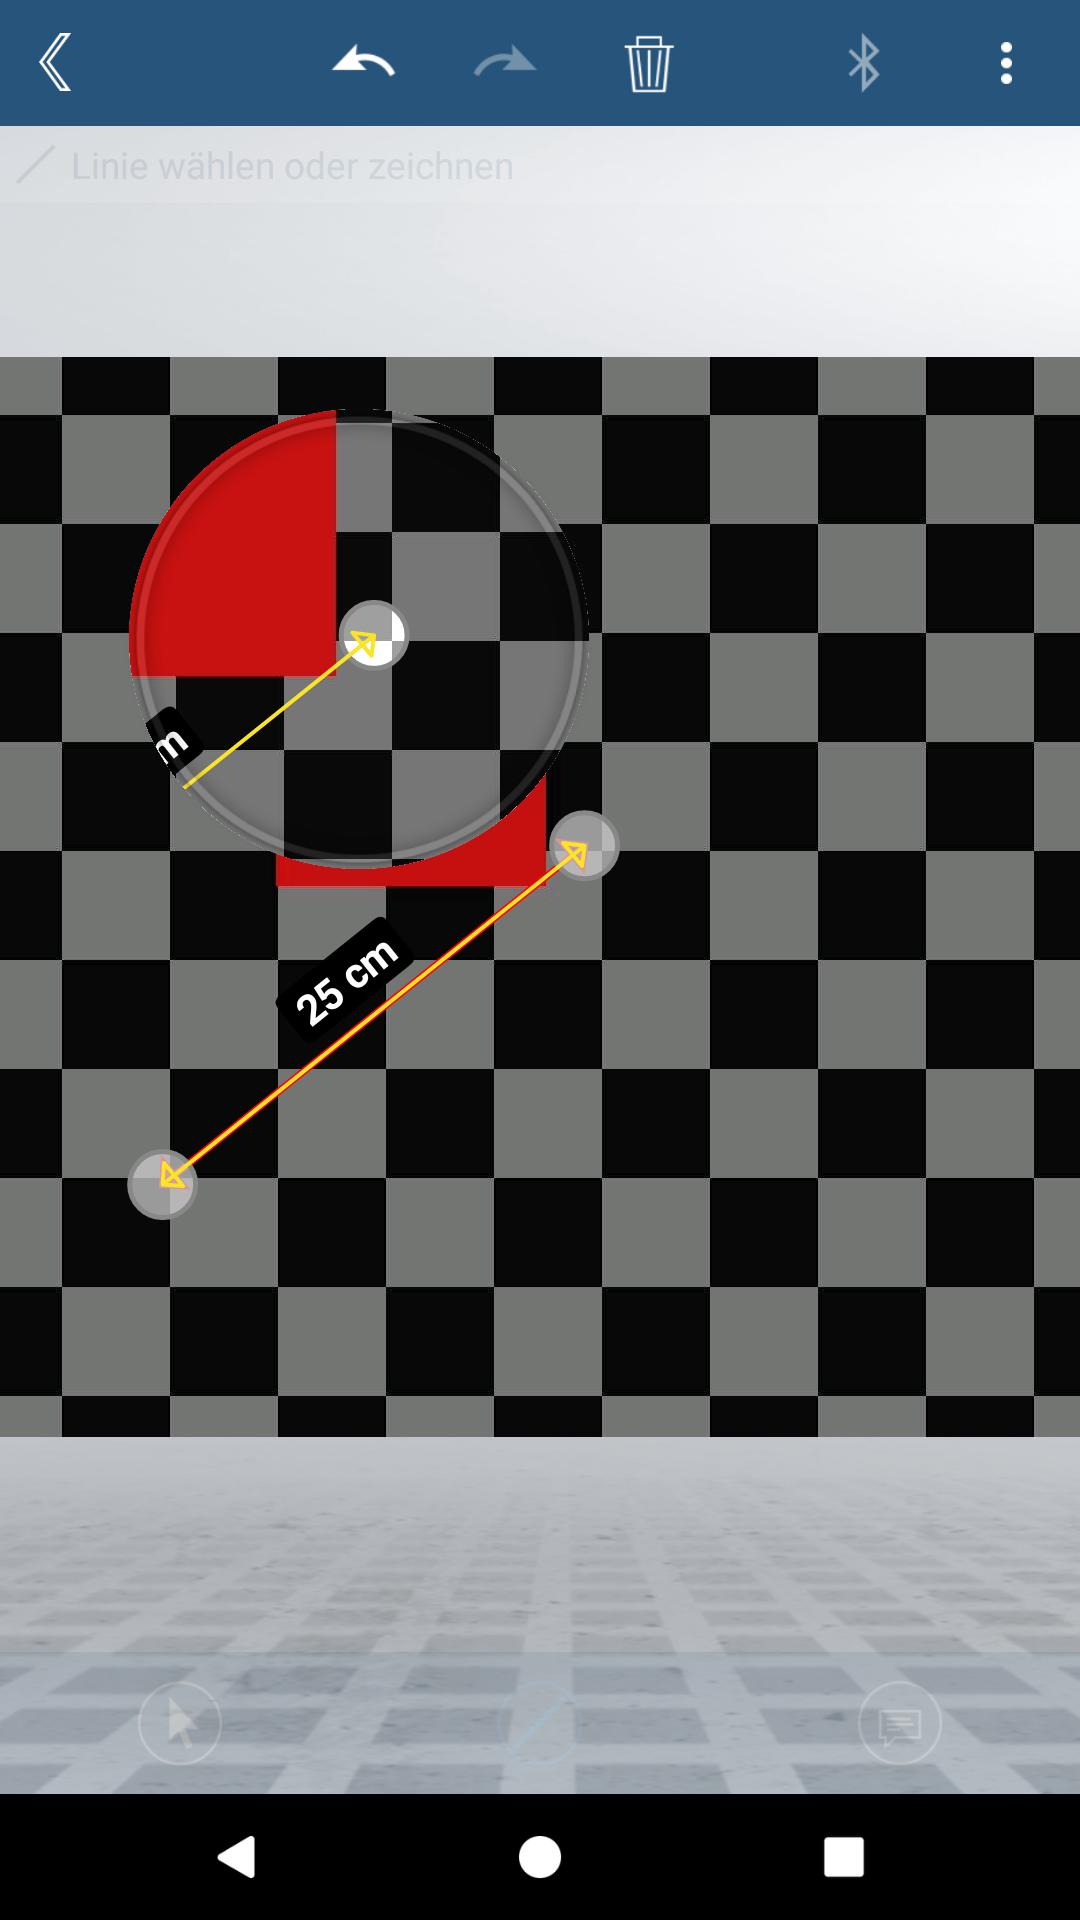
\includegraphics[keepaspectratio, width=0.4\textwidth]{bosch/lense}
  \caption{Zoom-Linse beim Zeichnen einer Form}
  \label{fig:blense}
\end{wrapfigure}

Einen ``Expertenmodus'', der es dem Benutzer ermöglicht, die App zu konfigurieren oder bestimmte Schritte abzukürzen, ist in der App nicht vorhanden (Nielsen~\autoref{itm:N7}).
So muss der Nutzer jedesmal, wenn er ein eine zuvor eingezeichnete Form beschriften will, in den Text-Modus wechseln, die gewünschte Form markieren, und anschließend die Messwerte eintragen.  \\

Markierte Formen werden durch die Verwendung einer anderen Farbe hervorgehoben.
Dies ermöglicht ein schnelles und effizientes Erfassen des Bildschirminhaltes, da sofort ersichtlich ist, welche Form zur Zeit ausgewählt ist (Nielsen~\autoref{itm:N12}). \\ 

Das Zeichnen von Formen durch das Klicken und anschließende Ziehen mit einem Finger auf dem Bildschirm ermöglicht eine einfache und effiziente Benutzung der App mit einer Hand (Nielsen~\autoref{itm:N17}).
Zusätzlich wird mit Hilfe einer Lupe, die sich beim Zeichnen stets neben dem Finger befindet, der Bereich unter dem Finger vergrößert dargestellt (siehe \autoref{fig:blense}).
Dies macht das Zeichnen von Formen nicht nur effizienter, sondern beugt auch Fehlern vor, da dieser Bereich sonst vom Finger des Benutzer bedeckt ist. \\

Des Weiteren kann die App zu jeder Zeit pausiert werden, ohne dass eingetragene Messwerte oder Formen verloren gehen (Nielsen~\autoref{itm:N11}). 
Dies ist besonders wichtig, wenn während der Benutzung der App bspw. ein Anruf angenommen werden muss. \\

Im Kontrast zu dem guten Umgang mit Unterbrechungen, führt die Rotation des Bildschirms vom Hoch- ins Querformat zu einer Drehung des Bildes in die Rotationsrichtung.
Hierdurch bleibt das Bild entgegen den Erwartungen nicht in der ursprünglichen Ausrichtung, in der es aufgenommen wurde, sondern dreht sich stets mit der Bildschirmausrichtung mit (Nielsen~\autoref{itm:N15}). \\
% \begin{figure}[h]
% \centering
% \begin{subfigure}[t]{0.4\textwidth}
% 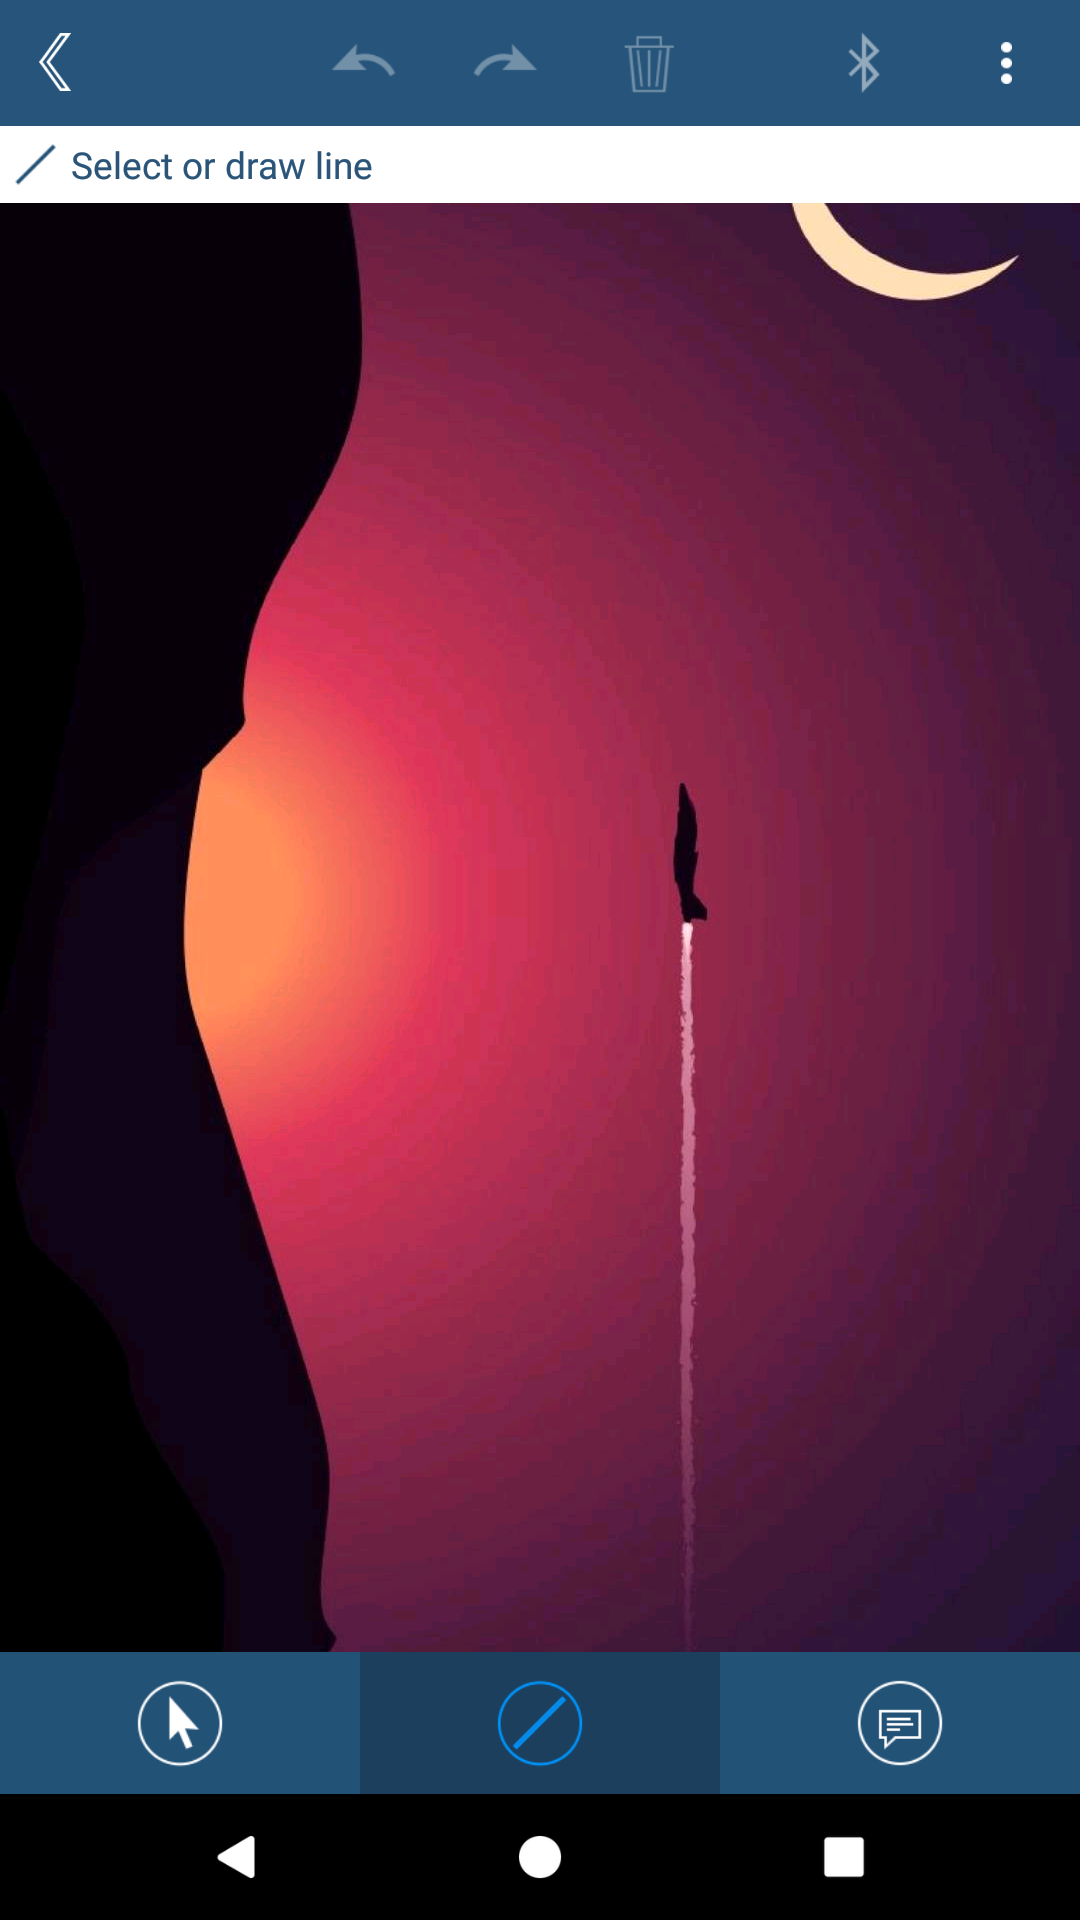
\includegraphics[keepaspectratio, width=\textwidth]{bosch/portrait}
% \caption{App im Hochformat}
% \end{subfigure}
% \begin{subfigure}[c]{0.4\textwidth}
% 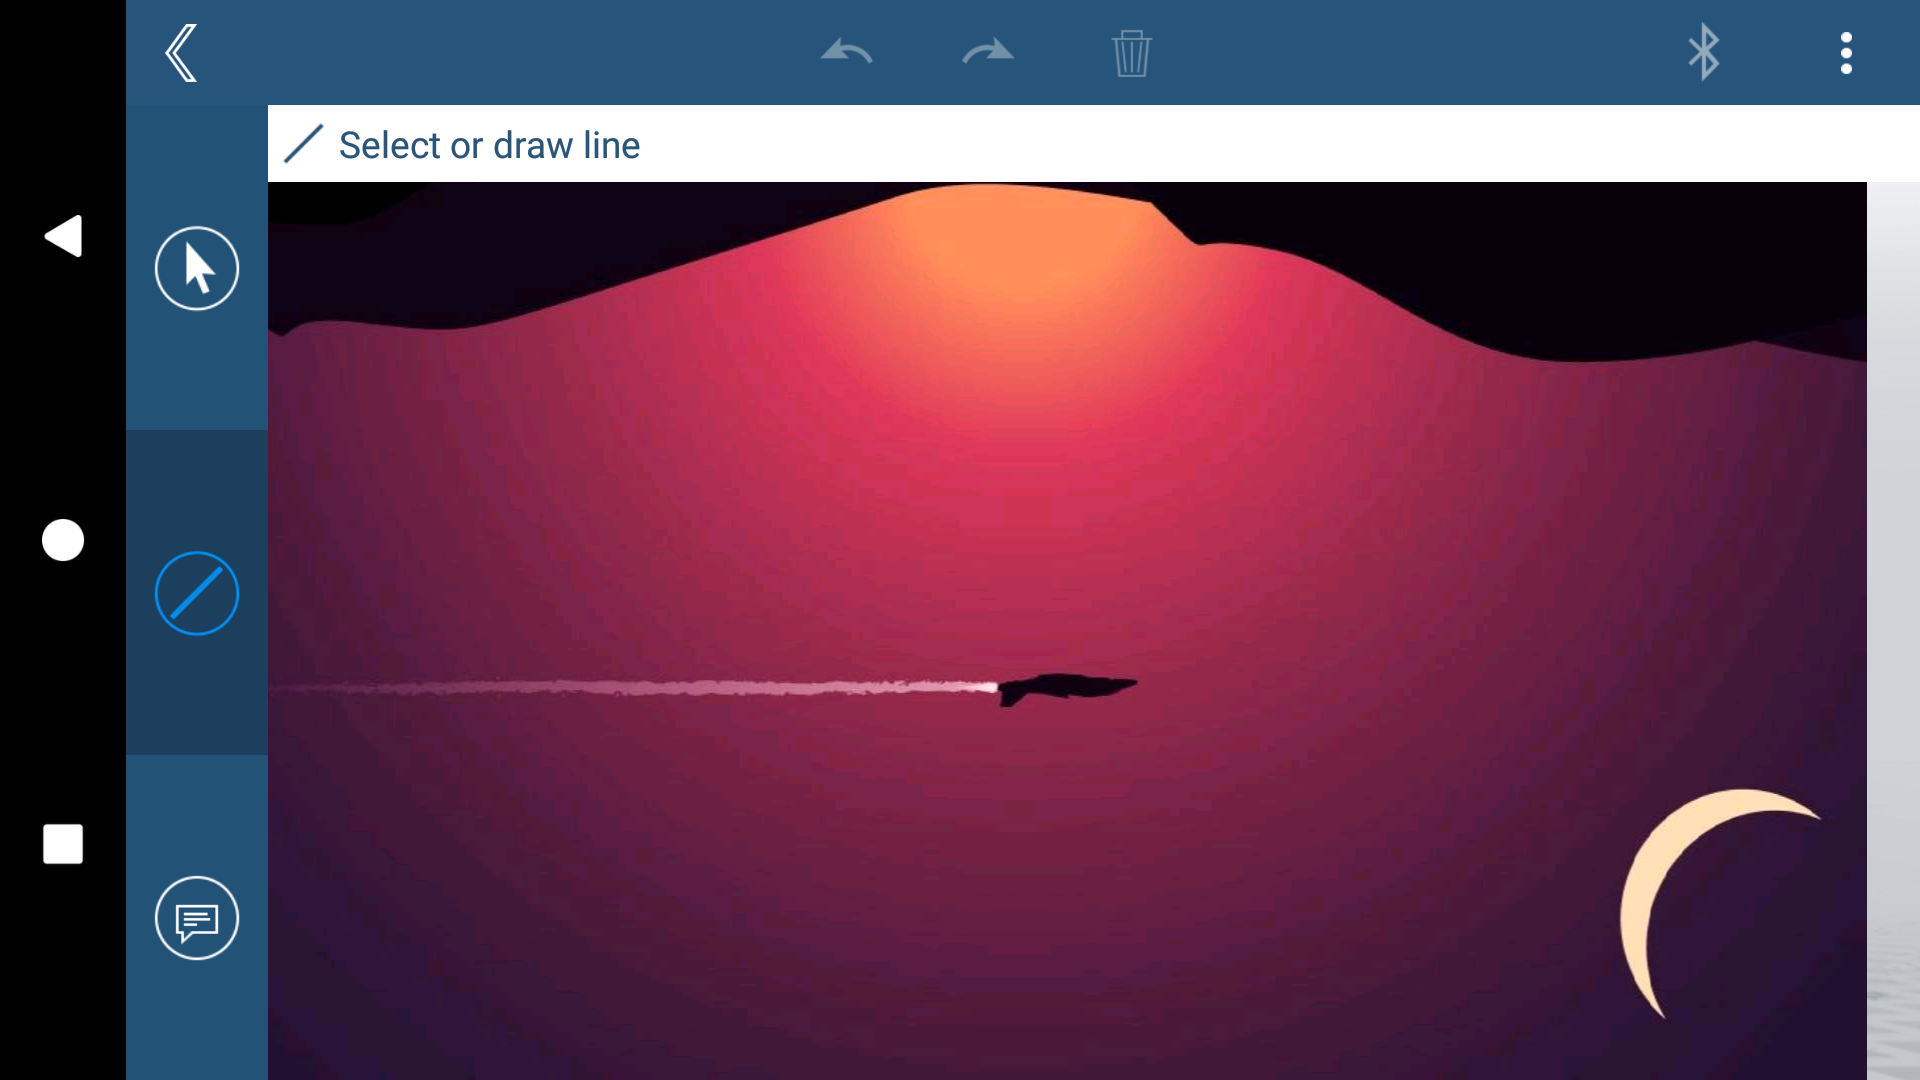
\includegraphics[keepaspectratio, width=\textwidth]{bosch/landscape}
% \caption{App im Querformat}
% \end{subfigure}
% \caption{App im Hochformat und im Querformat nach einer Rotation um 90 Grad gegen den Uhrzeigersinn}
% \label{fig:app14}
% \end{figure}

Wie bereits festgehalten, ermöglicht die App das Benutzen einer \emph{Drag-Geste} zum Zeichnen von Formen.
Die Gesten-Unterstützung zur Navigation im Bild ist jedoch nur nicht so gut umgesetzt worden.
So führt die fehlerhafte Umsetzung der \emph{Pinch-Geste} dazu, dass der Nutzer beim Zoomen des Bildes unabsichtlich eine Form zeichnet, wenn er zuvor im Zeichen-Modus ist (Nielsen~\autoref{itm:N16}).
Dieser Punkt wirkt sich negativ auf das Anwendungserlebnis aus, da hierdurch nach nahezu jeder Zoom-Aktion eine Undo-Aktion erzwungen wird, um die unabsichtlich-gezeichnete Form rückgängig zu machen (Nielsen~\autoref{itm:N13}). \\

Der Export des bearbeiteten Bildes führt dazu, dass alle zuvor eingetragenen Messwerte nicht mehr trivial auslesbar sind, da diese nicht mehr als Meta-Daten vorliegen (\autoref{itm:export}).
Zudem lässt sich die App nur schwer in eine bestehende Systemarchitektur integrieren, weil es keine Möglichkeit gibt, Bilder direkt in die App zu teilen, oder die annotierten Bilder inklusive der Meta-Daten für einen nachgelagerten Dienst aufzubereiten (\autoref{itm:integration}). \\

Zusammenfassend lässt sich festhalten, dass die App \mm{} von der Bosch GmbH die Usability-Heuristiken nach Nielsen größtenteils erfüllt.
Einzig bei der Benutzung von Gesten zum Zoomen im Bild und der Unterstützung von verschiedenen Bildschirmausrichtungen haben sich während der Evaluation Schwachstellen identifizieren lassen.
Besonders die fehlerhafte Gesten-Unterstützung und den damit verbundenen unabsichtlich-gezeichnete Formen ist ein Kritikpunkt, der das Nutzungserlebnis der App einschränkt.
Zudem lässt sich die Aufmaß-Funktion nicht in die bestehende Android-App integrieren, da es keine Möglichkeit gibt, annotierte Bilder inklusive der Meta-Daten an eine andere App zu teilen bzw. in einer anderen App aufgenommene Bilder direkt an \mm{} freizugeben.
Auch die eingetragenen Messwerte lassen sich im Nachhinein nur mühsam aus dem Bild extrahieren, da diese nicht mehr als Meta-Daten vorliegen, sodass die Weiterverarbeitung in einem nachgeschalteten Dienst wie einer \emph{API} nur schwer möglich sind.
